%%
\label{chap:case study}
While in the last chapters, the literature review of \ac{LCA} and existing \aclp{spdm} was presented, this chapter demonstrates the application of several \aclp{spdm} to an existing LCA database for chemical products provided by the company ``CarbonMinds GmbH''  \cite{CarbonMindsGmbH.2020} and that was developed at the Chair for Technical Thermodynamics at RWTH Aachen University. Initially, the goal and scope of the performed application of \aclp{spdm} will be defined. Subsequently, the general process used to generate the new simulation models based on \aclp{spdm} is explained. After that, the applied \aclp{spdm} are defined. Afterwards, the simulation model underlying the used LCA database called ``cm.chemicals'' \cite{CarbonMindsGmbH.2020} is broken down into the most important methodological aspects used in its creation that will then be discussed in detail. 

\section{Goal and Scope Definition}


The declared goal of this study is to assess the usability, accuracy and limitations of \aclp{spdm}, as well as the restrictions and pitfalls to avoid when using them in the context of existing LCA database frameworks.

The studied LCA database models the worldwide chemical industry. The scope includes 51 produced chemicals and 23 regions taking part in the production and trade of chemical products \cite{CarbonMindsGmbH.2020}. The list of products and regions can be found in Appendix \ref{appA}. The products include the 18 most important large-volume chemicals that account for 80 \% of the energy demand and make up more than 75 \% of the \acl{GHG} emissions of the chemical industry \cite{InternationalEnergyAgency.2013}. The mass and energy flows of 77 of the 194 production processes included in the named model are recalculated using two different \aclp{spdm}. This yields two new technology datasets that are then each integrated into the original LCA database separately. Thereby, two new LCA databases are created, containing technology data from one of the two \aclp{spdm}. These models are then used to calculate environmental impacts for the same chemical products and production processes as in the original database. 


\section{Database Framework}

In this chapter, all relevant methodological aspects used to generate the LCA database are named and briefly explained.


\paragraph{Technology Datasets}

The simulation model includes 194 engineering-level technology datasets representing the production processes of the part of the chemical industry represented in the model. For each flow occurring in the model, metadata from different sources is collected \cite{AmericanChemicalSociety.2020, Favre.2014, MerckKGaA.2020, RoyalSocietyofChemistry.2020}. This data is needed to calculate direct emissions of the processes due to the incineration of wastes.


\paragraph{Allocation Rules}

As chemical processes often have several products due to the underlying stoichiometry, \aclp{GWI} of single chemical products can only be calculated if the resulting multifunctional inventories are allocated. The relevant international standard \cite{InternationalOrganizationforStandardization.2006} proposes allocation by mass, energy or economic value ratios of the products. In accordance with this standard, we use mass ratio allocation, which is widely used by LCA practitioners \cite{EuropeanCommissionJointResearchCentreInstituteforEnvironmentandSustainability.2012c}.


\paragraph{Cut-off}
The same standard \cite{InternationalOrganizationforStandardization.2006} states that mass flows which constitute less then 5 mass-\% of the overall in- and outputs to the system can be cut-off to reduce the complexity of the simulation model. Additionally, not more than 5 mass-\% are cut-off from the model in total and all relevant substances are checked to make sure no important flow with high ecologic impact is cut-off.


\paragraph{Supply Processes}

All inputs needed but not produced within the system are supplied by processes from the Ecoinvent database version 3.6 \cite{Ecoinvent.2020}. For each region, a hierarchy of existing Ecoinvent regions is used to obtain a dataset that is as accurate as possible. A complete list of all used Ecoinvent processes can be found in Appendix \ref{app:ecoinvent}.


\paragraph{Production Shares}

One chemical can be produced via different synthesizing routes and several processes for the same route often exist. The shares of each technology in the model were calculated using market analysis data and then set to only produce at these fixed proportions.

\paragraph{Global Trade}
Publicly available data was used to calculate import and export flows of each chemical product to and from the world modeled to be the single trading partner of each region. This data was used to make sure products are only traded in these correct proportions. 







\section{Procedure of Model Generation}

In this chapter, the procedure used for the generation of the simulation models will be explained. It is divided into two parts to simplify its understanding. Figure \ref{fig:plan_1} shows the first part of this procedure and describes the generation of the new inventory datasets.

\begin{figure}[htp]
        \centering
        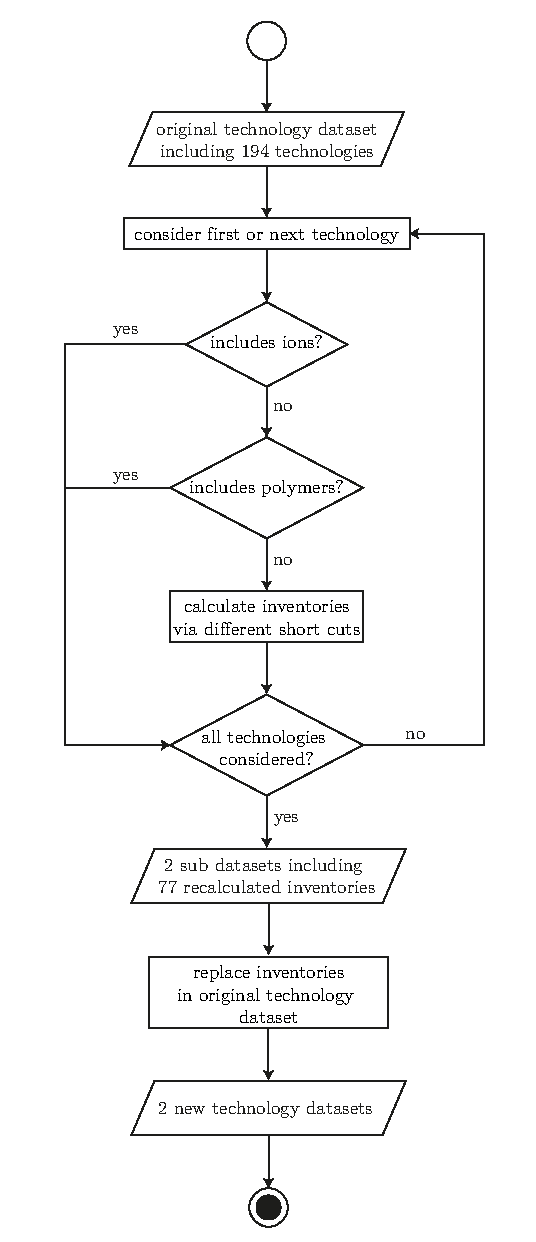
\includegraphics{images/plan_1.pdf}
        \caption{Part one of the model generation process: generating the new sets of inventories}
        \label{fig:plan_1}
\end{figure}

The core of the model underlying the LCA database are the 194 engineering-level technology datasets, each including mass and energy flows, characterizing the chemical processes used for the production of intermediates and the 51 chemicals referred to beforehand. These energy and mass flows are used as inventories of these processes for the calculation of the LCA database. Each one of them is considered individually to determine whether it can be recalculated using the automated \aclp{spdm}. These methods rely on thermodynamic properties such as their temperature-dependant enthalpy $h = h(T)$ and the standard enthalpy of formation $\Delta_f h^\standardstate$ to calculate reaction enthalpies used to estimate heat demands. These values can be determined using COSMO-RS, an equilibrium thermodynamics model and theory used to calculate chemical potentials of molecules in solutions \cite{Klamt.1995}. These are then used to calculate other thermodynamical properties. However, this method leads to high errors when used for ionic solutions, making the set of parameters used for the calculations a subject of recurring scientific publications \cite{Han.2018, Liu.2018}. For polymers, the procedure used by COSMO-RS cannot be applied due to the size of these chemical compounds. Alternatives exist, but report significant errors \cite{SoftwareforChemistry&Materials.2020}. Therefore, processes including ions and polymers are excluded from this study. If the process is not excluded from recalculation, its inventory is then determined with the two methods used in this study. This yields two sub datasets with 77 recalculated inventories. Each dataset including inventories calculated with one of the two \aclp{spdm}. Subsequently, these inventories replace the original ones in the LCA database. The second part starts with these new technology datasets as depicted in Figure \ref{fig:plan_2}.


\begin{figure}[htp]
        \centering
        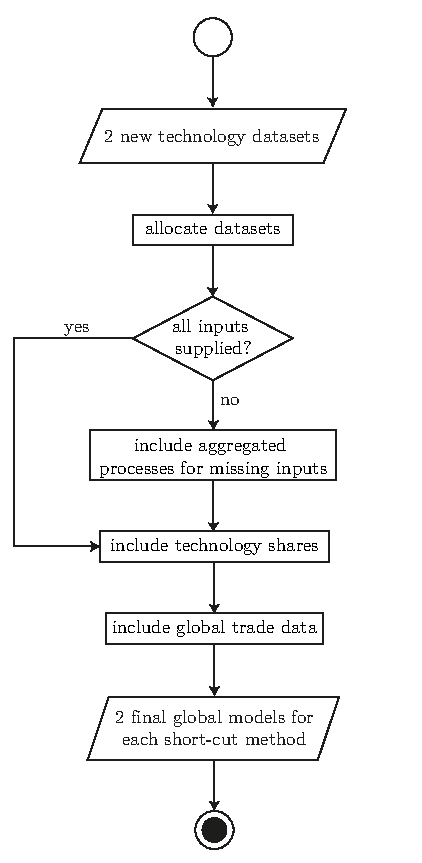
\includegraphics{images/plan_2.pdf}
        \caption{Part two of the model generation process: generating the new models}
        \label{fig:plan_2}
\end{figure}

The technology datasets are then allocated to solve the problem of multifunctionality, so that individual \aclp{GWI} for each chemical product can be calculated. The systems are then checked to identify whether all needed inputs are supplied. If there are unsupplied inputs, supply processes are added successively from the Ecoinvent database \cite{Ecoinvent.2020}. The production processes producing the same chemicals are then set to do so in fixed shares that reflect the real values varying from country to country. As the model also includes a global trade system, these trade flows are then added to the system. Thereby, two complete LCA databases are created, each modeling the worldwide chemical industry, but on the basis of different technology data.
\vspace{2cm}


\section{Applied Simplified Process Design Methods}

The individual methods used in this case study have all been described in detail in Chapter \ref{analysis-spdm}. However, the complete methods used in this case study are a combination of several \aclp{spdm} and are therefore defined in this Chapter.

\paragraph{Method 1: Stoichiometric Mass Flows and Reaction Enthalpy}
In the first method, the stoichiometric equations of the chemical processes are used with a yield of 95 \%, as described in Chapter \ref{stoichiometry}, and suggested by Hischier et. al. \cite{Hischier.2005} and the general rule of thumb proposed by Wells \cite{Wells.1991}. This yields the mass flows. Unconverted reactants are burned, creating direct emissions of the process. The heat use of the process is assumed to equal the reaction enthalpy of the process. The electric energy use is set to be the energy needed for pumps to supply the cooling water needed for the cooling of the reactor according to the reaction enthalpy.


\paragraph{Method 2: Stoichiometric Mass Flows and Ecoinvent's Default Energy Values}
The second method is a reproduction of the estimates used by Ecoinvent \cite{Hischier.2005} in case of few known information about a chemical process, as described in Chapter \ref{gendorf}. Mass inputs are stoichiometric with a yield of 95 \% and subsequent burning of unreacted educts. As default energy values, a use of 2 MJ steam and 0.33 kWh electric energy per kg of output chemical are estimated as suggested by Hischier et. al. \cite{Hischier.2005}. In contrast to the above mentioned method, no fugitive emissions are taken into account.



